% !TEX root = master_thesis.tex
\documentclass[12pt,maitrise]{dms}
\usepackage[utf8]{inputenc}
\usepackage[T1]{fontenc}
\usepackage{csquotes}
\usepackage[style=numeric, sorting=none, backend=biber, url=false, citestyle=numeric-comp]{biblatex}
\addbibresource{master_thesis.bib}

\usepackage{lmodern}
\DeclareSymbolFont{largesymbols}{OMX}{cmex}{m}{n}
\raggedbottom

\francais % or
%%\anglais
%%
%%\usepackage[english,frenchb]{babel}

\def\sloppy{%
  \tolerance 500%  %9999 dans LaTeX ordinaire, mauvaise idée.
  \emergencystretch 3em%
  \hfuzz .5pt
  \vfuzz\hfuzz}
\sloppy   %appel de \sloppy pour le document
%%\fussy  %ou \fussy

%% Packages 
\usepackage{graphicx,amssymb,subfigure}
\usepackage{amssymb}
\usepackage{subfigure}
\usepackage{physics}
\usepackage{xcolor}
\usepackage{url}
\usepackage[labelfont=bf, width=\linewidth]{caption}
\usepackage{hyperref} 
\definecolor{darkblue}{rgb}{0.0, 0.0, 0.5}
\hypersetup{colorlinks=true,allcolors=darkblue}
\usepackage{hypcap}   
\usepackage{bookmark} 
\usepackage{bm}
\usepackage{tikz}
\usetikzlibrary{arrows.meta, shadows, positioning, shapes.geometric}


\AtBeginDocument{%                 
  \setlength{\abovedisplayskip}{6pt}%
  \setlength{\belowdisplayskip}{6pt}%
  \setlength{\abovedisplayshortskip}{3pt}%
  \setlength{\belowdisplayshortskip}{3pt}%
}

%%\hypersetup{
%%  pdftitle = {Vers la simulation du spectre Raman résonant du graphène avec des défauts à partir des premiers principes},
%%  pdfauthor = {Grégoire Barrette},
%%  pdfsubject = {Calcul des propriétés de matériaux à l'aide de la théorie de la fonctionnelle de la densité},
%%  pdfkeywords = {Graphène, théorie de la fonctionnelle de la densité, spectroscopie Raman, interaction lumière-matière, interaction électron-phonon, physique de la matière condensée, défauts, calculs ab initio, théorie de la fonctionnelle de la densité perturbative, fonctions de Wanniers, self-énergie.}
%%}

%\newtheorem{cor}{\corollaryname}[section]
%\newtheorem{theo}[cor]{\theoremname}
%\newtheorem{prop}[cor]{Proposition}
%\newtheorem{lem}[cor]{\lemmaname}
%\theoremstyle{definition}
%\newtheorem{deff}[cor]{\definitionname}
%\newtheorem{ex}[cor]{\examplename}
%\newtheorem{rem}[cor]{\remarkname}
%\newtheorem{algo}[cor]{\algoname}


%%%
%%% Si vous préférez que les corollaires, définitions, théorèmes,
%%% etc. soient numérotés séparément, utilisez plutôt un bloc de
%%% commandes de la forme :
%%%

\newtheorem{cor}{\corollaryname}[section]
\newtheorem{deff}{\definitionname}[section]
\newtheorem{ex}{\examplename}[section]
\newtheorem{lem}{\lemmaname}[section]
\newtheorem{prop}{Proposition}[section]
\newtheorem{rem}{\remarkname}[section]
\newtheorem{theo}{\theoremname}[section]

\numberwithin{equation}{section}
\numberwithin{table}{chapter}
\numberwithin{figure}{chapter}

%%\makeindex

%% \usepackage[onehalfspacing]{setspace}
 % ou
\renewcommand{\baselinestretch}{1.286} %Interligne et demi (environ 18pt (12pt+6pt) entre les lignes)

%%%%%%%%%%%%%%%%%%%%%%%%%%%%%%%%%%%%%%%%%%%%%%%%%%%%%%%%%%%%
%%%%%%%%%%%%%%%%%%%%%%%%%%%%%%%%%%%%%%%%%%%%%%%%%%%%%%%%%%%%
%%%%%%%%%%                                     %%%%%%%%%%%%%
%%%%%%%%%% D é b u t    d u    d o c u m e n t %%%%%%%%%%%%%
%%%%%%%%%%                                     %%%%%%%%%%%%%
%%%%%%%%%%%%%%%%%%%%%%%%%%%%%%%%%%%%%%%%%%%%%%%%%%%%%%%%%%%%
%%%%%%%%%%%%%%%%%%%%%%%%%%%%%%%%%%%%%%%%%%%%%%%%%%%%%%%%%%%%
\begin{document}
\pagenumbering{roman}

%%------------------------------------------------- %
%%              pages i et ii                       %
%%------------------------------------------------- %
\title{Vers la simulation du spectre Raman résonant du graphène avec des défauts à partir des premiers principes}

\author{Grégoire Barrette}

\copyrightyear{2026}

\department{Département de physique}

\date{31 août 2026} 

\sujet{Physique}

\president{Nom du président du jury}

\directeur{Michel Côté}

%%\codirecteur{Nom du 1er codirecteur}         % s'il y a lieu
%%\codirecteurs{Nom du 2e codirecteur}         % s'il y a lieu

\membrejury{Nom du membre de jury}

\pdfbookmark[chapter]{Couverture}{PageUn}

%\maketitle
%\maketitle

%%------------------------------------------------- %
%%                Résumé.                           %
%%------------------------------------------------- %
%
\francais
\chapter*{Résumé}

Résumé (un maximum de 250 mots (1 page) pour les mémoires et 500 mots (2 pages) pour les thèses).

{\bf Mots-cl\'es :} graphène, spectroscopie Raman résonante, théorie de la fonctionnelle de la densité, couplage électron-phonon, couplage électron-défaut, fonctions de Wannier, théorie de la fonctionnelle de la densité perturbative, calculs \textit{ab initio}, physique de la matière condensée.

%%------------------------------------------------- %
%%                  Abstract                        %
%%------------------------------------------------- %
%\anglais
\chapter*{Abstract}

Abstract (maximum 250 words (1 page) for master thesis and 500 words (2 pages) for PhD thesis).

{\bf Keywords:} Graphene, resonant Raman spectroscopy, density functional theory, electron-phonon coupling, electron-defect coupling, Wannier functions, density functional perturbation theory, \text{ab initio} calculations, condensed matter physics.

%%------------------------------------------------- %
%%             Table des matières                   %
%%------------------------------------------------- %
\francais
\cleardoublepage
\pdfbookmark[chapter]{\contentsname}{toc} 
%\tableofcontents

%\cleardoublepage
%\listoftables

%\cleardoublepage
%\listoffigures

%%%%%%%%%%%%%%%%%%%%%%%%%%%%%%%%%%%%%
%% LISTE DES SIGLES ET ABRÉVIATION %
%%%%%%%%%%%%%%%%%%%%%%%%%%%%%%%%%%%%%
%\chapter*{Liste des sigles et des abréviations}
\def\coldeux{\relax}
\def\linestretch{3pt}

\begin{twocolumnlist}{.2\textwidth}{.7\textwidth}
 BvK & Born-von-Karman, se référant aux conditions de bord de Born-von-Karman ou le cristal de Born-von-Karman\\
 BZ & Zone de Brillouin, de l'anglais \textit{Brillouin Zone}\\
 DFT & Théorie de la fonctionnelle de la densité, de l'anglais
      \textit{Density Functional Theory}\\
 DFPT & Théorie de la fonctionnelle de la densité perturbative, de l'anglais \textit{Density Functional Perturbation Theory}\\
 FFT & Transformée de Fourier rapide, de l'anglais \textit{Fast Fourier Transform}\\
 GGA & Approximation du gradient généralisé, de l'anglais \textit{Generalized Gradient Approximation}\\
 DMFT & Théorie du champ moyen dynamique, de l'anglais \textit{Dynamical Mean Field Theory}\\
 HK & Hohenberg et Kohn, se référant aux théorèmes de Hohenberg et Kohn\\
 IBZ & Zone de Brillouin irréductible, de l'anglais \textit{Irreducible Brillouin Zone}\\
 KB & Kleinman et Bylander, se référant à la forme séparable de Kleinman et Bylander pour les pseudo-potentiels à conservation de norme\\
 KS & Kohn-Sham, se référant à la méthode de Kohn-Sham\\
 LDA & Approximation de la densité locale, de l'anglais \textit{Local Density Approximation}\\
 MLWF & Fonction de Wannier maximalement localisée, de l'anglais \textit{Maximally Localized Wannier Fonction}\\
 MP & Monkhorst-Pack, se référant à la grille de points-$\kv$ de Monkhorst-Pack\\
 NC & Conservation de la norme, de l'anglais \textit{Norm-Conserving}\\
 NSCF & Méthode du champ non-auto-cohérent, de l'anglais \textit{Non Self Consistent Field}\\
 ONCV & Conservation de norme optimisé de Vanderbilt, se référant aux pseudo-potentiels à conservation de norme optimisé de Vanderbilt (de l'anglais \textit{Optimized Norm-Conserving Vanderbilt})\\
 PBE & Perdew-Burke-Ernzerhof, se référant à la fonctionnelle d'échange-corrélation Perdew-Burke-Ernzerhof\\
 SCF & Méthode du champ auto-cohérent, de l'anglais \textit{Self Consistent Field}\\
 WF & Fonction de Wannier\\
 XC & Échange-corrélation, se référant à la fonctionnelle ou l'énergie d'échange-corrélation\\
\end{twocolumnlist}

%%------------------------------------------------- %
%%              liste des symboles                  %
%%------------------------------------------------- %
%\chapter*{Liste des symboles}
\begin{twocolumnlist}{.2\textwidth}{.7\textwidth}
    & \large\textbf{Généraux}\\
    $e$ & Charge élémentaire : $1.60217663\times 10^{-19}$ C\\
    $\varepsilon_0$ & Permittivité du vide : $8.8541878188\times 10^{-12}$ F m$^{-1}$\\
    $\hbar$ & Constante de Planck réduite : $1.054571817\times 10^{-34}$ J s\\
    $k_B$ & Constante de Boltzmann : $1.380649\times 10^{-23}$ m$^2$ kg s$^{-2}$ K$^{-1}$\\
    $T$ & Température en kelvins\\
    $\beta$ & Inverse de l'énergie thermique associée à la température : $\beta = 1 /k_BT$\\
    & \\

    & \large\textbf{Réseau cristallin}\\
    $\av_i$ & Vecteurs primitifs du réseau cristallin\\
    $\bv_i$ & Vecteurs primitifs du réseau réciproque du cristal\\
    $\Gv$ & Vecteurs du réseau réciproque du cristal\\
    $\Omega_\text{BvK}$ & Volume du cristal (ou du super-cristal de Born-von-Karman)\\
    $\Omega_\text{uc}$ & Volume de la cellule primitive\\
    $\Omega_\text{sc}$ & Volume de la super-cellule\\
    $N_\text{cells}$ & Nombre de cellules unitaires dans la super-cellule\\
    $N_\text{uc}$ & Nombre de cellules primitives dans le cristal\\ 
    $\Rv_l$ & Vecteurs du réseau cristallin qui identifient la cellule primitive $l$ \\
    $\bm{\tau}_\alpha$ & Position de l'atome $\alpha$ dans une cellule unitaire\\
    & \\

    & \large\textbf{Électrons}\\
    $\kv$ & Vecteur d'onde ou quasi-moment d'un électron\\
    $n$ & Indice de bande d'un électron\\
    $\varepsilon_{n\kv}$ & Énergie d'un électron dans le formalisme de Kohn-Sham\\
    $\ket{\psi_{n\kv}}$ & État quantique de Bloch d'un électron dans le formalisme de Kohn-Sham\\
    $\ket{u_{n\kv}}$ & Partie périodique de l'état de Bloch d'un électron\\
    $\ket{n\kv}$ & État quantique d'une onde plane électronique\\
    $C_{n\kv}(\Gv)$ & Coefficient de l'expansion en ondes planes des états de Bloch électroniques\\
    $\hat{c}^\dag_{n\kv}\,(\hat{c}_{n\kv})$ & Opérateur de création (destruction) d'un électron\\

    & \\

    & \large\textbf{Phonons et photons}\\
    $\qv$ & Vecteur d'onde ou quasi-moment d'un phonon ou d'un photon\\
    $\lambda$ & Polarisation d'un photon\\
    $\nu$ & Branche d'un phonon\\
    $\mathbf{e}_{\lambda\qv}$ & Vecteur de polarisation d'un photon\\
    $\mathbf{e}_{\nu\qv}$ & Vecteur de polarisation d'un phonon \\
    $\omega_{\qv}$ & Fréquence d'un photon\\
    $\omega_{\nu\qv}$ & Fréquence d'un phonon\\
    $\hat{a}_{\lambda\qv}^\dag\,(\hat{a}_{\lambda\qv})$ & Opérateur de création (destruction) d'un photon\\
    $\hat{b}_{\nu\qv}^\dag\,(\hat{b}_{\nu\qv})$ & Opérateur de création (destruction) d'un phonon\\
    $\hat{A}_{\nu\qv}$ & Opérateur proportionnel aux déplacements d'un phonon : $\hat{A}_{\nu\qv}=\hat{b}_{\nu\qv}+\hat{b}^\dag_{\nu-\qv}$\\
    & \\

    & \large\textbf{Couplage}\\
    $g_{nm\lambda}(\kv,\qv)$ & Élément de matrice de couplage électron-photon\\
    $g_{nm\nu}(\kv,\qv)$ & Élément de matrice de couplage électron-phonon\\
    $M_{nm}(\kv,\kv')$ & Élément de matrice de couplage électron-défaut\\
    & \\

    & \large\textbf{Fonctions de Green et \textit{self}-énergie} \\
    $\mathcal{D}_{\nu\qv}(i\nu_j)$ & Fonction de Green de Matsubara phononique aux fréquences de Matsubara\\
    $\mathcal{D}^{(0)}_{\nu\qv}(i\nu_j)$ & Fonction de Green de Matsubara phononique libre aux fréquences de Matsubara\\
    $\mathcal{G}_{n\kv}(i\omega_j)$ & Fonction de Green de Matsubara électronique aux fréquences de Matsubara\\
    $\mathcal{G}^\text{ed}_{n\kv}(i\omega_j)$ & Fonction de Green de Matsubara électronique due aux défauts aux fréquences de Matsubara\\
    $\mathcal{G}^\text{eph}_{n\kv}(i\omega_j)$ & Fonction de Green de Matsubara électronique due phonons aux fréquences de Matsubara\\
    $\mathcal{G}^{(0)}_{n\kv}(i\omega_j)$ & Fonction de Green de Matsubara électronique libre aux fréquences de Matsubara\\
    $\bar{\mathcal{G}}^\text{ed}_{n\kv}(i\omega_j)$ & Fonction de Green de Matsubara électronique moyenée pour une collections de défauts aux fréquences de Matsubara\\
    $i\omega_j$ & Fréquence de Matsubara fermionique\\
    $i\nu_j$ & Fréquence de Matsubara bosonique\\
    $\Pi_{\nu\qv}(\omega)$ & \textit{Self}-énergie phononique due aux interactions avec les électrons\\
    $\Sigma^\text{ed}_{n\kv}(\omega)$ & \textit{Self}-énergie électronique due aux interactions avec les défauts\\
    $\Sigma^\text{eph}_{n\kv}(\omega)$ & \textit{Self}-énergie électronique due aux interactions avec les phonons\\
    $S(\beta, 0)$ & Matrice $S$ dans le formalisme de Matsubara\\
    $T_{mn}(\kv',\kv)$ & Matrice $T$ pour le couplage des électrons avec un seul défaut\\

    & \\
    & \large\textbf{Hamiltoniens}\\
    $\hat{H}$ & Hamiltonien général\\
    $\hat{H}_0$ & Hamiltonien libre général\\
    $\hat{H}_\text{e}$ & Hamiltonien électronique\\
    $\hat{H}_\text{ed}$ & Hamiltonien de couplage électron-défaut\\
    $\hat{H}_\text{eem}$ & Hamiltonien de couplage électron-photon\\
    $\hat{H}_\text{em}$ & Hamiltonien des photons libres\\  
    $\hat{H}_\text{eph}$ & Hamiltonien de couplage électron-phonon\\
    $\hat{H}_\text{i}$ & Hamiltonien ionique\\
    $\hat{H}_\text{int}$ & Hamiltonien d'interaction général\\
    $\hat{H}_\text{KS}$ & Hamiltonien de Kohn-Sham dans le formalisme de la théorie de la fonctionnelle de la densité\\
    $\hat{H}_\text{ph}$ & Hamiltonien des phonons libres\\
\end{twocolumnlist}

%%------------------------------------------------- %
%%            Remerciements                         %
%%------------------------------------------------- %
%\chapter*{Remerciements}

Je remercie plusieurs individus.


\NoChapterPageNumber
\cleardoublepage
\pagenumbering{arabic}

%%%%%%%%%%%%%%%%%%%%%%%%%%%%%%%%%%%%%%%%%%%%%%%%%%%%%
%%                                                  %
%%             TEXTE DU MÉMOIRE                     %
%%                                                  %
%%%%%%%%%%%%%%%%%%%%%%%%%%%%%%%%%%%%%%%%%%%%%%%%%%%%%

%\chapter{Introduction}
Introduction du mémoire.
% !TEX root = ../master_thesis.tex
\chapter{Préliminaires théoriques}\label{chap:théorie}

Dans ce chapitre, nous détaillons les fondements théoriques nécessaires à la compréhension de la spectroscopie Raman et des travaux de ce mémoire. Nous partons de l'Hamiltonien général d'un solide cristallin et des approximations qui permettent de découpler le problème en une partie électronique et une partie ionique. Nous verrons comment résoudre ces deux parties, introduirons les fonctions de Wannier et présenterons brièvement le couplage entre la lumière et les électrons du système. 

\section{Hamiltonien général d'un solide cristallin}\label{sec:2.1}

Toute l'information d'un système quantique est contenue dans la fonction d'onde $\Psi$ et sa connaissance nous donne accès à toutes les propriétés du système. Pour la trouver, il faut résoudre l'équation de Schrödinger
\begin{equation}
    H\Psi = E\Psi,
\end{equation}
où $H$ est l'opérateur qui représente l'énergie totale du système et $E$ est l'énergie totale. Les systèmes qui nous intéressent sont des solides cristallins composés d'atomes arrangés périodiquement sur un réseau cristallin. Ces atomes sont constitués d'électrons de valence, responsables des propriétés physiques et chimiques d'intérêt, et d'électrons de c\oe ur, fortement liés aux noyaux et chimiquement inertes. Ces derniers sont traités conjointement avec les noyaux pour former des ions de masses $M_{I}$ et de pseudo-charge $Z_{I}$. Tous ces constituants sont électriquement chargés et interagissent mutuellement par l'entremise d'un potentiel de Coulomb. L'Hamiltonien général qui représente un ensemble de $N_e$ électrons et $N_i$ ions est donné par
\begin{equation}
\begin{split}
    H &= -\sum_{i=1}^{N_e}\frac{\hbar^2}{2m_e}\nabla_i^2
        -\sum_{I=1}^{N_i}\frac{\hbar^2}{2M_I}\nabla_I^2
        +\frac{1}{2}\sum_{\substack{IJ \\ I\neq J}}^{N_i}
        \frac{Z_IZ_Je^2}{4\pi\varepsilon_0|\rv_I-\rv_J|} \\
      &\quad +\frac{1}{2}\sum_{\substack{ij \\ i\neq j}}
        \frac{e^2}{4\pi\varepsilon_0|\rv_i-\rv_j|}+\sum_{i=1}^{N_e}V_\text{ext}(\rv_i),
\end{split}
\label{eqn:c2_H_general}
\end{equation}
où nous reconnaissons, dans l'ordre, l'énergie cinétique des électrons, l'énergie cinétique des ions, la répulsion Coulombienne ion-ion, la répulsion Coulombienne électron-électron et l'attraction Coulombienne électron-ion, encodée dans le potentiel externe $V_\text{ext}(\rv)$ qui sera remplacé par un pseudo-potentiel dans la section~\ref{sec:PP}. Dans ce mémoire, des termes supplémentaires à cet Hamiltonien seront introduits aux chapitres~\ref{chap:défauts} et~\ref{chap:eph} pour décrire le couplage des électrons avec les défauts dans le système et les vibrations des ions \textit{i.e.} les phonons.

Bien qu'il soit relativement facile de poser le problème, sa résolution l'est beaucoup moins. Nous faisons face ici à un problème à $N=N_e+N_i$ corps couplés par l'interaction Coulombienne, dont la fonction d'onde $\Psi(\{\rv_i\},\{\rv_I\})$ dépend simultanément de $3N$ variables. Le nombre de paramètres nécessaires pour représenter cette fonction d'onde croît exponentiellement avec le nombre de particules $N$ : pour un système de seulement 10 particules discrétisé sur une grille de $10\times10\times10=10^3$ points, il faudrait $(10^3)^{10}=10^{30}$ valeurs -- soit davantage que tout ce que l'humanité a jamais enregistré~\cite{hilbertWorldsTechnologicalCapacity2011}. Pour un solide macroscopique avec $\sim 10^{23}$ atomes par cm$^3$~\cite{alloulIntroductionPhysicsElectrons2011a}, une solution directe de l'équation de Schrödinger est tout simplement hors de portée, de par la complexité cauchemardesque du problème. Il est nécessaire d'introduire des approximations (section~\ref{sec:2.1.1}) et d'exploiter les symétries du système (section~\ref{sec:2.1.2}) pour réduire la complexité du problème.

\subsection{Approximation de Born-Oppenheimer}\label{sec:2.1.1}

Une première simplification majeure provient du rapport entre la masse des ions et celle des électron ($M_I/m_e \approx 10^4$--$10^5$) : les électrons, beaucoup plus légers, s'adaptent quasi-instantanément aux déplacements ioniques et restent dans leur état fondamental pour chaque configuration ionique. Nous disons qu'ils suivent les ions \textit{adiabatiquement}. C'est l'approximation adiabatique de Born-Oppenheimer~\cite{bornZurQuantentheorieMolekeln1927}, qui permet de découpler le problème en séparant la fonction d'onde totale en un produit d'une fonction d'onde électronique et d'une fonction d'onde ionique
\begin{equation}
    \Psi(\{\rv_i\},\{\rv_I\})=\psi(\{\rv_i\};\{\rv_I\})\phi(\{\rv_I\}),
    \label{eqn:c2_BO}
\end{equation}
où $\psi(\{\rv_i\};\{\rv_I\})$ est la fonction d'onde électronique, résolue pour des positions ioniques $\{\rv_I\}$ fixes (qui jouent le rôle de paramètres) et $\phi(\{\rv_I\})$ est la fonction d'onde ionique\footnote{Bien sûr, dans la vraie vie, les ions ne sont pas fixes. Ils oscillent autour d'une position d'équilibre à cause de la température notamment. Cela a un effet sur les électrons, qui sera traité perturbativement dans le chapitre~\ref{chap:eph} sur le couplage électron-phonon. Nous discutons des limitations de l'approximation adiabatique à la fin de cette section.}. L'Hamiltonien se sépare également en deux parties : $H=H_e+H_i$. Le problème électronique, résolu pour des positions ioniques fixes, est
\begin{equation}
    H_e\psi(\{\rv_i\};\{\rv_I\})=E_e\psi(\{\rv_i\};\{\rv_I\}),
    \label{eqn:c2_problème_électronique}
\end{equation}
avec l'Hamiltonien électronique
\begin{equation}
    H_e=\underbrace{-\sum_{i=1}^{N_e}\frac{\hbar^2}{2m_e}\nabla_i^2}_{\equiv T}+\underbrace{\frac{1}{2}\sum_{\substack{ij \\ i\neq j}}^{N_e}\frac{e^2}{4\pi\varepsilon_0|\rv_i-\rv_j|}}_{\equiv V_\text{int}}+\sum_{i=1}^{N_e}V_\text{ext}(\rv_i),
    \label{eqn:c2_He}
\end{equation}
Une fois le problème électronique résolu, le problème ionique devient
\begin{equation}
    H_i\phi(\{\rv_I\})=E\phi(\{\rv_I\}),
    \label{eqn:c2_problème_ionique}
\end{equation}
avec l'Hamiltonien ionique
\begin{equation}
    H_i = -\sum_{I=1}^{N_i}\frac{\hbar^2}{2M_I}\nabla_I^2+\underbrace{\frac{1}{2}\sum_{\substack{IJ \\ I\neq J}}^{N_i}\frac{Z_IZ_Je^2}{4\pi\varepsilon_0|\rv_I-\rv_J|}+E_e}_{\equiv U}.
    \label{eqn:c2_Hi}
\end{equation}
où le potentiel ionique effectif $U$ regroupe la répulsion Coulombienne entre les ions et l'énergie de l'état fondamental électronique $E_e$, qui assure la cohésion du solide. L'approximation de Born-Oppenheimer ayant découplé le problème en deux parties, nous nous consacrons dans la section~\ref{sec:2.2} à la résolution de la partie électronique via la théorie de la fonctionnelle de la densité, puis dans la section~\ref{sec:2.3} à la partie ionique via la théorie de la fonctionnelle de la densité perturbative.

Finalement, l'approximation de Born-Oppenheimer a ses limites. Elle néglige par construction le couplage entre les électron et les vibrations des ions (le couplage électron-phonon), responsable entre autres de la diffusion Raman. Elle devient également invalide lorsque le gap électronique est plus petit que l'énergie caractéristique des vibrations ioniques~\cite{pisanaBornOppenheimerBreakdownGraphene2007}. Cette condition est systématiquement violée dans le graphène, puisque le gap est nul au point $\Kv$ de la zone de Brillouin. Il y a deux façons de corriger ces effets non-adiabatiques : ne pas faire l'approximation adiabatique et utiliser le formalisme de Born-Huang~\cite{bornDynamicalTheoryCrystal1998} ou bien ajouter les corrections non-adiabatiques perturbativement à l'approximation de Born-Oppenheimer. Nous employons cette dernière stratégie dans le chapitre~\ref{chap:défauts} pour traiter les corrections non-adiabatiques, qui sont non-négligeables dans le graphène.

\subsection{Symétries du réseau cristallin et théorème de Bloch}\label{sec:2.1.2}

Une autre simplification majeure vient du fait que les solides cristallins sont des systèmes hautement symétriques. Ils sont des répétitions périodiques d'une unité de base : la cellule unitaire. Nous identifions les cellules unitaires par les vecteurs du réseau cristallin $\Rv_\ell$, où $\ell$ est un triplet d'entiers $(n_1,n_2,n_3)$
\begin{equation}
    \Rv_\ell = n_1\av_1+n_2\av_2+n_3\av_3.
    \label{eqn:c2_Rl}
\end{equation}
Ici, les vecteurs $\av_i$ sont les vecteurs primitifs du réseau cristallin et définissent la cellule unitaire. Comme toutes les cellules du solide sont les mêmes, il suit que l'Hamiltonien est invariant sous une translation discrète d'un vecteur du réseau. Il est généralement favorable de travailler de l'espace réciproque -- l'ensemble de points $\kv$ -- pour exploiter la symétrie de translation d'un système. À cet effet, nous introduisons le réseau réciproque, qui est un ensemble de points dans l'espace réciproque étiquetés par les vecteurs du réseau réciproque $\Gv$
\begin{equation}
    \Gv = m_1\bv_1+m_2\bv_2+m_3\bv_3,
    \label{eqn:c2_G}
\end{equation}
où les $m_i$ sont des entiers et les $\bv_i$ sont les vecteurs primitifs du réseau réciproque qui satisfont la condition suivante
\begin{equation}
    \av_i\cdot\bv_j=2\pi\delta_{ij}.
\end{equation}
Il fut démontré par Félix Bloch~\cite{blochUeberQuantenmechanikElektronen1929}, alors doctorant sous la supervision de Werner Heisenberg, que la fonction d'onde d'une particule évoluant avec un Hamiltonien invariant sous translation discrète se factorise en un produit d'une onde plane et une fonction périodique
\begin{equation}
    \psi_{n\kv}=e^{i\kv\cdot\rv}u_{n\kv}(\rv),
    \label{eqn:c2_bloch_thm}
\end{equation}
où la fonction périodique de Bloch possède la même invariance sous une translation discrète d'un vecteur du réseau que l'Hamiltonien
\begin{equation}
    u_{n\kv}(\rv+\Rv_\ell)=u_{n\kv}(\rv),
    \label{eqn:c2_unk}
\end{equation}
un résultat connu sous le nom de théorème de Bloch. Les vecteurs $\kv$ sont conservés modulo un vecteur du réseau réciproque $\Gv$, une conséquence directe de la symétrie de translation discrète. De ce fait, il est possible de restreindre l'espace réciproque à la première zone de Brillouin (BZ, de l'anglais \textit{Brillouin Zone}), soit l'ensemble de points $\kv$ plus proches de $\Gv=\mathbf{0}$ que de tout autre vecteur du réseau réciproque. N'importe quel point $\kv$ en dehors de la première BZ peut être replié dans la première BZ par une translation d'un vecteur $\Gv$. Pour distinguer les multiples solutions au même $\kv$ de la première BZ, nous avons introduit l'indice de bande $n$. Finalement, comme la fonction $u_{n\kv}(\rv)$ est la même dans toutes les cellules, il est possible de résoudre le problème dans une cellule unitaire seulement et reproduire la solution dans tout le solide par périodicité. En d'autres termes, au lieu de résoudre le problème pour le solide en son entier avec un nombre \textit{a priori} infini d'électrons et d'ions, le théorème de Bloch nous permet de restreindre le problème à une cellule unitaire avec un nombre fini d'électrons et d'ions, ce qui réduit énormément la complexité du calcul. 

Hormis la symétrie de translation discrète, les solides cristallins possèdent également des symétries ponctuelles -- rotations, inversions et réflexions -- qui forment le groupe de points. De plus, pour les systèmes non-magnétiques, la symétrie d'inversion du temps rend les points $\kv$ et $-\kv$ équivalents. Ces deux symétries combinées permettent de restreindre les calculs à la zone de Brillouin irréductible (IBZ, de l'anglais \textit{Irreducible Brillouin Zone}), soit le sous-ensemble de points $\kv$ non-équivalents. Pour le graphène, dont le groupe de points est $D_{6h}$~\cite{dresselhausPhysicalPropertiesCarbon1998,castronetoElectronicPropertiesGraphene2009}, l'IBZ représente $1/24$ de la BZ totale, ce qui réduit considérablement le coût numérique des intégrations sur la BZ.

\section{Partie électronique : théorie de la fonctionnelle de la densité}\label{sec:2.2}

Dans cette section nous nous attaquons au problème électronique défini par l'Hamiltonien de l'équation \ref{eqn:c2_He}, que nous répétons ici par souci d'exhaustivité
\begin{equation}
    H_e = T+V_\text{int}+\sum_{i=1}^{N_e}V_\text{ext}(\rv_i).
\end{equation}
Le problème, qui ne contient plus les degrés de liberté ioniques, est \textit{a priori} plus facile à résoudre que le problème initial. Cependant, en inspectant l'Hamiltonien de plus près, nous voyons tout de suite que ce n'est pas le cas : le deuxième terme, \textit{i.e.} la répulsion électrique entre les électrons, couple tous les électrons du système entre eux et les mêmes arguments utilisés à la section \ref{sec:2.1} s'appliquent malheureusement ici. Les physiciens et chimistes ont développé de nombreuses méthodes pour traiter ce problème : des méthodes basées sur les fonctions d'onde comme Hartree~\cite{hartreeWaveMechanicsAtom1928,hartreeWaveMechanicsAtom1928a} et Hartree-Fock~\cite{fockNaeherungsmethodeZurLoesung1930,slaterNoteHartreesMethod1930,diracQuantumMechanicsManyelectron1929}, sur les fonctions de Green~\cite{martinTheoryManyParticleSystems1959,AbrikosovAAGorkov} ou encore des méthodes stochastiques comme le Monte-Carlo quantique \cite{ceperleyGroundStateElectron1980}. Parmi toutes ces méthodes, une a révolutionné le domaine de la structure électronique : la théorie de la fonctionnelle de la densité (DFT, de l'anglais \textit{Density Functional Theory}). Les arguments présentés ici suivent ceux du livre de référence de Richard M. Martin \cite{martinElectronicStructureBasic2004} et ceux de l'ouvrage de Steven M. Girvin et Kun Yang \cite{girvinModernCondensedMatter2019}. 

\subsection{Théorèmes de Hohenberg et Kohn}\label{sec:2.2.1}

Les fondements de la DFT ont été édifiés par Pierre Hohenberg et Walter Kohn (HK) dans leur article de 1964~\cite{hohenbergInhomogeneousElectronGas1964} où ils énoncent et prouvent les deux théorèmes ci-bas. Le premier théorème de HK se lit : 
\begin{theo}
    \label{thm:hk1}
    Pour n'importe quel système de particules en interaction sujettes à un potentiel externe $V_\text{ext}(\rv)$, le potentiel externe est uniquement déterminé, sauf pour une constante, par la densité de l'état fondamental $n_0(\rv)$.
\end{theo}
\noindent
Ce théorème est facilement prouvé par l'absurde en invoquant le principe variationnel de la mécanique quantique. On peut imaginer comment un potentiel externe peut donner lieu à une certaine configuration électronique et donc une densité $n(\rv)$. Le premier théorème HK démontre que le chemin inverse est tout aussi vrai, \textit{i.e.} il y a une bijection entre le potentiel externe et la densité électronique de l'état fondamental. Un corollaire très important découle de ce premier théorème:
\begin{cor}
    \label{cor:hk1}
    Comme l'Hamiltonien est complètement déterminé par la densité électronique hormis un décalage constant de l'énergie, il suit que les fonctions d'onde à plusieurs corps pour tous les états (fondamental et excités) sont déterminées. Par conséquent, toutes les propriétés du système sont complètement déterminées par la densité de l'état fondamental $n_0(\rv)$.
\end{cor}
\noindent
C'est une avancée conceptuelle et théorique exceptionnelle puisque au lieu de déterminer les propriétés d'un système à partir de la fonction d'onde $\psi(\{\rv_i\})$, une fonction de $3N_e$ variables dont la complexité croit exponentiellement avec le nombre d'électrons $N_e$ (qui est un nombre extrêmement grand pour un solide macroscopique), nous pouvons déterminer les propriétés du système à partir de la densité de l'état fondamental $n(\rv)$, une fonction qui ne dépend que de trois variables, peu importe le nombre d'électrons! À première vue cela est étonnant, car la densité électronique est normalement calculée à partir de la fonction d'onde
\begin{equation}
    n(\rv)=N_e\int d^3\rv_2\dots d^3\rv_{N_e}|\psi(\rv,\rv_2,\dots,\rv_{N_e})|^2,
\end{equation}
où l'intégration se fait sur toutes les coordonnées électroniques sauf une ($\rv\equiv\rv_1$ ici, qui est un choix arbitraire). De plus, le premier théorème de HK ne fournit pas de prescription pour déterminer la densité sans faire appel à la fonction d'onde à plusieurs corps. À ce stade, il semble que nous n'ayons pas fait beaucoup de progrès. Le deuxième théorème de HK et son corollaire se lisent : 
\begin{theo}
    \label{thm:hk2}
    Il est possible de définir une fonctionnelle universelle pour l'énergie $E[n]$ en termes de la densité électronique $n(\rv)$ qui est valide pour n'importe quel $V_\text{ext}(\rv)$. Pour chaque $V_\text{ext}(\rv)$, l'énergie exacte de l'état fondamental du système est le minimum global de cette fonctionnelle et la densité qui la minimise est celle de l'état fondamental $n_0(\rv)$. 
\end{theo}
\begin{cor}
    \label{cor:hk2}
    La fonctionelle E[n] à elle seule suffit à déterminer l'énergie et la densité exactes de l'état fondamental. 
\end{cor}
\noindent
Le terme \textit{fonctionnelle} ici fait référence à une application de l'espace des fonctions vers les nombres réels, contrairement aux \textit{fonctions} qui sont des applications des nombres réels vers des nombres réels. Nous utilisons des crochets pour écrire une fonctionnelle $E[n]$ et des parenthèses pour écrire une fonction $n(\rv)$. L'idée est que puisque toutes les propriétés du système sont déterminées par la densité selon le premier théorème de HK, toutes ces propriétés, incluant l'énergie totale, peuvent être écrites comme étant une fonctionnelle de la densité $n(\rv)$
\begin{align}
    E[n]&=\bra{\psi[n]}T+V_\text{int}\ket{\psi[n]}+\int d^3\rv\,V_\text{ext}(\rv)n(\rv),\notag\\
    &= T[n]+V_\text{int}[n]+\int d^3\rv\,V_\text{ext}(\rv)n(\rv),\notag\\
    &\equiv F_\text{HK}[n]+\int d^3\rv\,V_\text{ext}(\rv)n(\rv).
\end{align}
Ici, nous avons défini la fonctionnelle de HK, $F_\text{HK}\equiv T+V_\text{int}$, qui ne dépend que de l'énergie cinétique et l'énergie d'interaction électron-électron du système d'électrons. Comme cette fonctionnelle ne dépend pas de paramètre externe, elle est universelle dans le sens qu'elle est la même pour tous les systèmes d'électrons, peu importe le potentiel externe : la configuration des ions, un champ électrique, ou toute autre perturbation externe. En théorie, nous pouvons déterminer la densité de l'état fondamental en minimisant la fonctionnelle d'énergie $E[n]$ (théorème de HK II), puis utiliser cette densité pour calculer n'importe quelles propriétés du système (théorème de HK I), pourvu que nous connaissions la forme de la fonctionnelle $F_\text{HK}$. En pratique, la forme exacte de $F_\text{HK}$ n'est pas connue et étant donné qu'elle est la même pour tous les systèmes d'électrons interagissants, il est attendu que cette fonctionnelle soit d'une complexité fantastique. Il va sans dire que quiconque trouverait sa forme exacte meriterait certainement un prix Nobel. Le deuxième théorème de HK nous fournit donc une prescription pour déterminer la densité de l'état fondamental du système, mais n'offre aucune piste pour calculer la fonctionnelle $F_\text{HK}$ dans laquelle toute la complexité du problème à été reléguée. Encore une fois, il semble que nous n'ayons pas fait beaucoup de progrès.

\subsection{Méthode de Kohn-Sham}\label{sec:2.2.2}

Quelques mois après la publication de l'article de HK, Walter Kohn et Lu Jeu Sham (KS) publient un article~\cite{kohnSelfConsistentEquationsIncluding1965} en 1965 dans lequel ils proposent une approche pratique pour contourner le problème de la fonctionnelle universelle $F_\text{HK}$ et posent les équations qui sont à la base des calculs DFT actuels.

\noindent\textbf{Système auxiliaire de Kohn-Sham}

Le génie de KS se trouve dans l'idée d'introduire un système auxiliaire -- le système auxiliaire de KS -- de $N_e$ électrons \textit{sans interaction} soumis à un potentiel effectif local $V_\text{eff}(\rv)$ choisi de sorte que la densité électronique de ce système auxiliaire soit identique à celle du système réel en interaction et de résoudre le problème dans ce système auxiliaire. Rappelons que $N_e$ signifie maintenant le nombre d'électrons dans une cellule unitaire et non dans le solide en son entier. Le premier théorème de HK  garantit l'existence de ce potentiel effectif puisqu'il établit une bijection entre le potentiel externe et la densité de l'état fondamental. Ce système est beaucoup plus facile à traiter puisque en l'absence d'interaction entre les électrons, la fonction d'onde à plusieurs corps se factorise en un déterminant de Slater de $N_e$ fonctions d'onde à un corps $\psi_{n\kv}(\rv)$. La correspondance entre le système auxiliaire et le vrai système à plusieurs corps est illustré dans la figure~\ref{fig:ks}. La densité du système auxiliaire n'est que la somme du carré des fonctions d'onde à un corps
\begin{equation}
    \label{eqn:c2_nKS}
    n(\rv) = 2\sum_{n\kv}^{\text{occ}}|\psi_{n\kv}(\rv)|^2=n_0(\rv),
\end{equation}
où nous avons explicité que la densité du système auxiliaire doit être la même que le système réel en interaction. Le facteur de 2 tient compte de la dégénerescence en spin des états électroniques pour un système non polarisé en spin. La somme court sur tous les états électroniques étiquetés par $(n\kv)$ occupés. L'énergie cinétique d'un système d'électron non-interagissant est aussi calculable exactement : elle correspond à la somme de l'énergie cinétique de chaque particule 
\begin{equation}
    \label{eqn:c2_TS}
    T_\text{S}=-\frac{\hbar^2}{2m_e}2\sum_{n\kv}^{\text{occ}}\bra{\psi_{n\kv}}\nabla^2\ket{\psi_{n\kv}}.
\end{equation}
KS ont aussi inclus l'énergie d'interaction électron-électron de manière effective via l'énergie d'Hartree~\cite{hartreeWaveMechanicsAtom1928,hartreeWaveMechanicsAtom1928a,fockNaeherungsmethodeZurLoesung1930}
\begin{equation}
    \label{eqn:c2_EH}
    E_\text{H}[n]=\frac{1}{2}\int d^3\rv\,d^3\rv'\,\frac{e^2}{4\pi\varepsilon_0}\frac{n(\rv)n(\rv')}{|\rv-\rv'|}.
\end{equation}
qui correspond à l'énergie classique de Coulomb de 
l'interaction d'une densité de charge avec elle-même. C'est une 
approximation de champ moyen de la vraie interaction électron-électron. Il est évident que nous faisons des erreurs en remplaçant $T[n]$ et $V_\text{int}[n]$ par $T_\text{S}[n]$ et $E_\text{H}[n]$ dans la fonctionnelle universelle $F_\text{HK}$. Pour pallier ces erreurs, KS ont introduit la fonctionnelle d'échange-corrélation (XC) $E_\text{XC}[n]$ qui contient toutes les corrections d'interaction électron-électron qu'il faut apporter à $T_\text{S}[n]$ et $E_\text{H}[n]$ pour retomber sur la fonctionnelle $F_\text{HK}$ exacte. Dans la méthode de KS, la fonctionnelle universelle s'écrit
\begin{equation}
    \label{eqn:c2_FHK_KS}
    F_\text{HK}[n]=T_\text{S}[n]+E_\text{H}[n]+E_\text{XC}[n],
\end{equation}
de sorte que l'énergie totale s'écrit maintenant
\begin{equation}
    \label{eqn:c2_EKS}
    E_\text{KS}[n]=T_\text{S}[n]+E_\text{H}[n]+E_\text{XC}[n]+\int d^3\rv\,V_\text{ext}(\rv)n(\rv).
\end{equation}
Nous avons atteint notre objectif qui était de traiter les complications engendrées par la fonctionnelle universelle. Cependant, les célébrations sont de courte durée, car il est bien clair que toute la complexité du problème à plusieurs corps en interaction a encore une fois été reléguée, cette fois dans la fonctionnelle XC $E_\text{XC}[n]$. En théorie, la formulation de la DFT est exacte, pourvu que nous trouvions la forme exacte de la fonctionnelle XC. En pratique, la forme exacte de cette fonctionnelle n'est pas connue, mais il a été constaté qu'il existe des approximations à la fonctionnelle XC qui donnent de très bons résultats pour une grande variété de systèmes. Nous en discutons à la section~\ref{sec:XC}. Finalement, un mot sur la signification d'\textit{échange} et \textit{corrélation}. Les électrons sont soumis à deux types de corrélations : la \textit{corrélation} proprement dite, qui est due à l'interaction Coulombienne au-delà de l'approximation de champ moyen (Hartree), et l'\textit{échange}, une corrélation d'origine purement statistique due à la nature fermionique des électrons imposée par le principe d'exclusion de Pauli. 

\begin{figure}[t]
    \centering
    \begin{tikzpicture}[
    box/.style={rectangle, draw=black, rounded corners,
                fill=gray!15, minimum width=2.8cm,
                minimum height=0.8cm, align=center},
    arrow/.style={->, >=stealth, thick},
    darrow/.style={<->, >=stealth, thick}
]

% ---- Titres ----
\node[box, minimum width=6.2cm] at (-3.5, 2.5)
    {\textbf{Système interagissant}};
\node[box, minimum width=6.2cm] at (3.5, 2.5)
    {\textbf{Système auxiliaire de KS}};

% ---- Ligne du haut ----
\node[box] (vext)   at (-5.2,  1.2) {$V_\text{ext}(\rv)$};
\node[box] (n0l)    at (-1.8,  1.2) {$n_0(\rv)$};
\node[box] (n0r)    at ( 1.8,  1.2) {$n_0(\rv)$};
\node[box] (vks)    at ( 5.2,  1.2) {$V_\text{KS}(\rv)$};

% ---- Ligne du bas ----
\node[box] (psii)   at (-5.2, -0.6) {$\Psi_i(\{\rv\})$};
\node[box] (psi0)   at (-1.8, -0.6) {$\Psi_0(\{\rv\})$};
\node[box] (phiine) at ( 1.8, -0.6) {$\psi_{i=1,N_e}(\rv)$};
\node[box] (phii)   at ( 5.2, -0.6) {$\psi_i(\rv)$};

% ---- Flèches horizontales haut ----
\draw[darrow] (vext.east) -- (n0l.west)
    node[midway, above] {\small HK};
\draw[darrow] (n0l.east)  -- (n0r.west)
    node[midway, above] {\small KS};
\draw[darrow] (n0r.east)  -- (vks.west)
    node[midway, above] {\small HK$_0$};

% ---- Flèches verticales ----
\draw[arrow] (vext.south)   -- (psii.north);
\draw[arrow] (psi0.north)   -- (n0l.south);
\draw[arrow] (phiine.north) -- (n0r.south);
\draw[arrow] (vks.south)    -- (phii.north);

% ---- Flèches horizontales bas ----
\draw[arrow] (psii.east)  -- (psi0.west);
\draw[arrow] (phii.west)  -- (phiine.east);

\end{tikzpicture}
    \caption[Représentation schématique du système auxiliaire de Kohn-Sham.]{Représentation schématique du système auxiliaire de Kohn-Sham. La notation HK$_0$ désigne les théorèmes de HK appliqués au système auxiliaire non-interagissant. La flèche double KS donne la connexion entre les deux systèmes de sorte que chaque boîte du schéma soit reliée à toutes les autres. En conséquence, la solution du système auxiliaire donne, en théorie, toutes les propriétés du système à plusieurs corps en interaction. Figure adaptée de \cite{martinElectronicStructureBasic2004}.}
    \label{fig:ks}
\end{figure}

\noindent\textbf{Équations de Kohn-Sham}

Le deuxième théorème de HK garantit que l'énergie de l'état fondamental du système auxiliaire de KS est le minimum de la fonctionnelle d'énergie $E_\text{KS}[n]$ définie dans l'équation \eqref{eqn:c2_EKS} et la densité qui la minimise est celle de l'état fondamental $n_0(\rv)$. En minimisant cette fonctionnelle par rapport aux fonctions d'onde sous la contrainte d'orthonormalisation $\bra{\psi_{n\kv}}\ket{\psi_{n'\kv'}}=\delta_{nn'}\delta_{\kv\kv'}$, nous arrivons aux fameuses équations de KS
\begin{equation}
    \label{eqn:c2_KS}
    H_\text{KS}\psi_{n\kv}=\varepsilon_{n\kv}\psi_{n\kv},
\end{equation}
où $\varepsilon_{n\kv}$ est l'énergie de la fonction d'onde à un électron $\psi_{n\kv}$ et $H_\text{KS}$ est l'Hamiltonien effectif à un électron de KS
\begin{equation}
    \label{eqn:c2_HKS}
    H_\text{KS}=-\frac{\hbar^2}{2m_e}\nabla^2+V_\text{KS}(\rv),
\end{equation}
avec le potentiel effectif de KS
\begin{align}
    \label{eqn:c2_VKS}
    V_\text{KS}(\rv)&=V_\text{ext}(\rv)+\frac{\delta E_\text{H}}{\delta n(\rv)}+\frac{\delta E_\text{XC}}{\delta n(\rv)}\notag\\
    &=V_\text{ext}(\rv)+V_\text{H}(\rv)+V_\text{XC}(\rv),
\end{align}
C'est la grande simplification de la méthode de KS: le problème à $N_e$ corps en interaction a été reformulé en $N_e$ équations indépendantes à une seule particule, dont la complexité varie linéairement avec $N_e$ plutôt qu'exponentiellement. C'est cette réduction qui rend les calculs DFT praticables.

Ces équations doivent cependant être résolues de manière auto-cohérente : le potentiel $V_\text{KS}(\rv)$ dépend de la densité $n(\rv)$ via $V_\text{H}(\rv)$ et $V_\text{XC}(\rv)$, qui est elle-même obtenue à partir des fonctions d'onde -- solutions des équations de KS. Nous détaillons cette procédure d'autocohérence (méthode SCF, de l'anglais \textit{Self-Consistent Field}) ainsi que son implémentation pratique dans la base d'ondes planes dans la section~\ref{sec:PW}.

Nous notons enfin que les valeurs propres $\varepsilon_{n\kv}$ des équations de KS n'ont pas de signification physique directe : ce sont des multiplicateurs de Lagrange introduits pour satisfaire la condition d'orthonormalisation des fonctions d'onde, et non l'énergie nécessaire pour ajouter ou retirer des électrons du système en interaction. La seule exception est la plus haute valeur propre occupée, qui correspond à moins l'énergie d'ionisation, un résultat connu sous le nom de théorème de Janak~\cite{janakProof1978}. En pratique, ces valeurs propres sont néanmoins utilisées pour calculer les structures de bandes et les densités d'états, un usage formellement abusif dont la manifestation la plus connue est la sous-estimation systématique du gap électronique par la DFT~\cite{perdewPhysicalContentExact1983,shamDensityFunctionalTheoryEnergy1983}.

Le succès extraordinaire de la méthode de KS tient à deux facteurs : la réduction du problème à plusieurs corps en équations découplées à une particule, et le succès remarquable des approximations pour la fonctionnelle XC $E_\text{XC}[n]$ discutées à la section~\ref{sec:XC}. Les articles de HK \cite{hohenbergInhomogeneousElectronGas1964} et de KS \cite{kohnSelfConsistentEquationsIncluding1965} sont encore aujourd'hui parmi les plus cités de la \textit{Physical Review}.

\subsection{Fonctionnelles d'échange-corrélation}\label{sec:XC}

Le choix de l'approximation pour la fonctionnelle d'échange-corrélation (XC) $E_\text{XC}[n]$ a une influence significative sur les résultats des calculs DFT. Les approximations disponibles sont organisées en une hiérarchie -- l'échelle de Jacob, introduite par Perdew \cite{perdewJacobsLadderDensity2001} et illustrée à la figure \ref{fig:jacob} -- où chaque échelon incorpore davantage d'information sur la densité électronique, gagnant en précision au prix d'un coût computationnel accru. Dans cette section, nous présentons brièvement les deux premiers échelons et justifions notre choix de fonctionnelle. 
\begin{figure}[h]
    \centering
    \begin{tikzpicture}[
    rung/.style={
        draw=black,
        fill=gray!15,
        rounded corners=4pt,
        minimum width=12cm,
        minimum height=1.0cm,
        align=center,
        font=\small
    },
    arrow/.style={
        -{Stealth[length=8pt]},
        line width=1.5pt
    },
    label/.style={
        font=\small,
        align=center
    }
]

% ---- rungs (bottom to top) ----
\node[rung] (lda)  at (0,0)
    {\textbf{LDA} --- approximation de la densité locale\\
     $n(\rv)$};

\node[rung,fill=darkblue!15] (gga)  at (0,1.5)
    {\textbf{GGA} --- approximation du gradient généralisé\\
     $n(\rv)$ et $\nabla n(\rv)$};

\node[rung] (mgga) at (0,3.0)
    {\textbf{meta-GGA} --- densité d'énergie cinétique\\
     $n(\rv), \nabla n(\rv)$ et $\tau(\rv)$};

\node[rung] (hyb)  at (0,4.5)
    {\textbf{Hybrides} --- échange exact\\};

\node[rung] (rpa)  at (0,6.0)
    {\textbf{RPA / Double hybrides} --- corrélation non-locale\\
     Fonctionnelles dépendant des états inoccupés};

% ---- ground and heaven ----
\node[draw=black, fill=gray!15, rounded corners=4pt,
      minimum width=12cm, minimum height=0.7cm,
      align=center, font=\small] (earth) at (0,-1.1)
    {Théorie de Hartree};

\node[draw=black, fill=gray!15, rounded corners=4pt,
      minimum width=12cm, minimum height=0.7cm,
      align=center, font=\small] (heaven) at (0,7.1)
    {Solution exacte};

% ---- ladder poles ----
\draw[line width=2pt, black] (-5.5,-0.75) -- (-5.5,6.75);
\draw[line width=2pt, black] ( 5.5,-0.75) -- ( 5.5,6.75);

% ---- vertical arrows ----
\draw[arrow, black] (-7.0,-0.55) -- (-7.0,6.75)
    node[midway, left=4pt, label]
    {Précision\\croissante};

\draw[arrow, black] (7.0,6.75) -- (7.0,-0.55)
    node[midway, right=4pt, label]
    {Coût\\décroissant};

\end{tikzpicture}
    \caption[L'échelle de Jacob des approximations pour la fonctionnelle d'échange-corrélation.]{L'échelle de Jacob des approximations pour la fonctionnelle d'échange-corrélation. Chaque échelon de l'échelle incorpore davantage d'information sur le système électronique gagnant en précision au prix d'un coût computationel accru. Le deuxième échelon est mis en évidence, car nous utilisons une fonctionnelle de ce niveau pour tous les calculs de ce mémoire. Figure adaptée de \cite{perdewJacobsLadderDensity2001}.}
    \label{fig:jacob}
\end{figure}


\noindent
\textbf{Premier échelon : approximation de la densité locale}

Le premier échelon de l'échelle de Jacob est l'approximation de la densité locale (LDA, de l'anglais \textit{Local Density Approximation}) proposée par Kohn et Sham eux-mêmes dans leur article fondateur de 1965 \cite{kohnSelfConsistentEquationsIncluding1965}. L'idée centrale de la LDA est d'approximer localement la fonctionnelle XC par celle d'un gaz d'électrons interagissants homogène de même densité $n$ 
\begin{equation}
    E_\text{XC}^\text{LDA}[n]=\int d^3\rv\,n(\rv)\,\varepsilon_\text{XC}^\text{hom}(n),
    \label{eqn:c1_LDA}
\end{equation}
où $\varepsilon_\text{XC}^\text{hom}(n)$ est la densité d'énergie d'échange-corrélation du gaz d'électrons homogène\footnote{Homogène signifie ici que la densité est la même partout dans le gaz : $n(\rv)=n$. La densité d'énergie d'échange-corrélation du gaz $\varepsilon_\text{XC}^\text{hom}(n)$ n'est pas une fonctionnelle, car $n$ n'est plus une fonction, d'où les parenthèses.}. Cette densité d'énergie peut être décomposée en une contribution d'échange et une contribution de corrélation : la partie d'échange est connue analytiquement \cite{martinElectronicStructureBasic2004}, tandis que la partie de corrélation a été calculée numériquement par Ceperley et Alder \cite{ceperleyGroundStateElectron1980} puis paramétrée par Perdew et Zunger \cite{perdewSelfinteractionCorrectionDensityfunctional1981}.

Malgré sa simplicité, la LDA connaît un succès remarquable pour les métaux et les semi-conducteurs. Elle souffre cependant de plusieurs limitations : elle tend à sous-estimer les constantes du réseau (\textit{overbinding}) \cite{perdewAtomsMoleculesSolids1992}, sous-estime systématiquement les gaps électroniques \cite{perdewPhysicalContentExact1983,shamDensityFunctionalTheoryEnergy1983} et ne peut décrire les interactions de van der Waals \cite{grimmeAccurateDescriptionVan2004,rapcewiczFluctuationAttractionCondensed1991} ni les systèmes à forte corrélation électronique \cite{BasisElectronTheory,imadaMetalinsulatorTransitions1998,anisimovBandTheoryMott1991,georgesDynamicalMeanfieldTheory1996}. Ces limitations ont motivé le développement du deuxième échelon.\\
\noindent
\textbf{Deuxième échelon : approximation du gradient généralisé et la PBE}

L'idée centrale de la GGA est d'aller au-delà de la LDA en incorporant non seulement la densité locale $n(\rv)$, mais aussi son gradient $\nabla n(\rv)$, afin de tenir compte de l'inhomogénéité de la densité électronique
\begin{equation}
    E_\text{XC}^\text{GGA}[n]=\int d^3\rv\,n(\rv)\,\left[\varepsilon_\text{X}^\text{hom}(n)\,F_\text{X}(n,\nabla n)+\varepsilon_\text{C}^\text{hom}(n)\,F_\text{C}(n,\nabla n)\right],
\end{equation}
où $F_\text{X}$ et $F_\text{C}$ sont les facteurs d'amplification adimensionnels pour l'échange et la corrélation respectivement qui encodent la correction due au gradient et $\varepsilon_\text{X/C}^\text{hom}(n)$ est de nouveau la densité d'énergie d'échange/corrélation d'un gaz d'électrons homogène. La fonctionnelle GGA la plus répandue est celle développée par Perdew, Burke et Ernzerhof\footnote{Matthias Ernzerhof est un professeur titulaire au département de chimie de l'Université de Montréal.} (PBE)~\cite{perdewGeneralizedGradientApproximation1996a}, dont les facteurs d'amplification sont construits à partir de conditions exactes connues sur la fonctionnelle XC, sans paramètres empiriques. Les expressions explicites de la PBE se trouvent dans l'annexe~\ref{annexe:pbe} et nous réferons le lecteur à l'article original pour les dérivations. Nous utilisons cette fonctionnelle pour tous les calculs de ce mémoire.

La PBE corrige l'\textit{overbinding} systématique de la LDA et donne de très bons résultats à moindre coût computationnel~\cite{kurthMolecularSolidstateTests1999,mounetFirstprinciplesDeterminationStructural2005a}, ce qui en fait une fonctionnelle de choix pour ce mémoire. Pour le graphène, la PBE décrit correctement les propriétés électroniques et vibrationnelles. En particulier, la PBE reproduit fidèlement le gap nul du graphène : les cônes de Dirac au point $\Kv$ de la zone Brillouin\footnote{Non pas parce que la PBE reproduit exactement les effets d'échange-corrélation, mais parce que les cônes de Dirac sont protégés par la symmétrie du réseau hexagonal. En effet, même un simple modèle \textit{tight-binding}, qui néglige complètement les interactions électron-électron, reproduit les cônes de Dirac. C'est une propriété d'origine purement géométrique.}. Les interactions de van der Waals, toujours absentes dans la PBE, sont négligeables pour le graphène monocouche étudié ici. De plus, les électrons $\pi$ des orbitales $p_z$ du carbone, qui dominent largement les propriétés électroniques du graphène, sont délocalisés et faiblement corrélés, ce qui rend la PBE tout à fait appropriée.  Les fonctionnelles des échelons supérieurs apportent des corrections négligeables aux systèmes de graphènes étudiés dans ce mémoire, à un coût computationnel prohibitif pour les super-cellules nécessaires à la modélisation des défauts, ce qui renforce notre choix de la PBE. L'article PBE \cite{perdewGeneralizedGradientApproximation1996a} est encore aujourd'hui l'un des plus cités de la \textit{Physical Review}.

Notons finalement que la sous-estimation du gap électronique demeure une limitation fondamentale de toutes les fonctionnelles locales ou semi-locales, incluant la PBE. Pour une description quantitative des intensités Raman résonantes, il sera probablement nécessaire de corriger les valeurs propres de Kohn-Sham à l'aide de l'approximation $GW$ \cite{hedinNewMethodCalculating1965,hybertsenElectronCorrelationSemiconductors1986}, qui traite les effets d'échange et de corrélation via la fonction de Green $G$ et l'interaction de Coulomb écrantée $W$, et qui donne des gaps qui sont en excellent accord avec l'expérience.

\subsection{Pseudo-potentiels}\label{sec:PP}

Le potentiel externe $V_\text{ext}(\rv)$, qui décrit l'interaction de Coulomb entre les électrons et les noyaux, diverge en $1/r$ au voisinage des ions. Cette singularité génère des états de c\oe ur fortement oscillants près des noyaux, auxquels les fonctions d'onde des électrons de valence héritent d'oscillations rapides afin de satisfaire à la condition d'orthonormalité. Ces électrons de c\oe ur, fortement liés aux noyaux et chimiquement inertes, contribuent peu aux propriétés d'intérêt et augmentent considérablement le coût des calculs. L'approximation des pseudo-potentiels~\cite{phillipsEnergyBandInterpolationScheme1958,phillipsNewMethodCalculating1959} résout ces deux problèmes simultanément : les électrons de c\oe ur sont absorbés dans les noyaux pour former les ions et leur effet sur les électrons de valence est encodé dans un pseudo-potentiel $V_\text{PP}(\rv)$ qui remplace le potentiel de Coulomb divergent par un potentiel plus lisse, réduisant à la fois le nombre d'électrons à traiter explicitement et la complexité des fonctions d'onde de valence.

On distingue principalement trois grandes catégories de pseudo-potentiels : les pseudo-potentiels à conservation de norme (NC, de l'anglais \textit{Norm-Conserving}) \cite{hamannNormConservingPseudopotentials1979}, les pseudo-potentiels \textit{ultrasoft} de Vanderbilt \cite{vanderbiltSoftSelfconsistentPseudopotentials1990} et la méthode des ondes augmentées projetées (PAW, de l'anglais \textit{Projector Augmented Waves}) de Blöchl \cite{blochlProjectorAugmentedwaveMethod1994}. Pour tous les calculs effectués dans ce mémoire nous utilisons des pseudo-potentiels de NC de la famille ONCV (de l'anglais \textit{Optimized Norm-Conserving Vanderbilt}) tirés de la bibliothèque PseudoDojo \cite{vansettenPseudoDojoTrainingGrading2018}, qui offrent un excellent compromis entre précision et efficacité computationnelle. Les pseudo-potentiels NC satisfont la condition de conservation de la norme
\begin{equation}
    \int_0^{r_c}dr\,|\psi_\ell^\text{PP}(r)|^2r^2=\int_0^{r_c}dr\,|\psi_\ell^\text{AE}(r)|^2r^2,
    \label{eqn:c2_nc}
\end{equation}
où $\psi_\ell^\text{AE}(r)$ est la fonction d'onde de valence que nous obtiendrions si nous résolvions les équations de KS avec le vrai potentiel de Coulomb et en traitant tous les électrons explicitement (l'indice AE vient de l'anglais \textit{All Electrons}), $\psi_\ell^\text{PP}(r)$ est la fonction d'onde obtenue en résolvant le problème dans l'approximation des pseudo-potentiels et $r_c$ est un rayon de coupure au-delà duquel les deux fonctions d'onde coïncident exactement. Cette condition garantit la bonne reproduction de la densité de charge dans la région de c\oe ur ainsi qu'une bonne transférabilité du pseudo-potentiel à différents environnements chimiques~\cite{hamannGeneralizedNormconservingPseudopotentials1989,troullierEfficientPseudopotentialsPlanewave1991}.

\noindent\textbf{Pseudo-potentiels ONCV et forme de Kleinman-Bylander}

Dans les codes DFT modernes, la forme séparable proposée par Kleinman et Bylander (KB)~\cite{kleinmanEfficaciousFormModel1982} pour les pseudo-potentiels NC est généralement employée, car elle réduit radicalement le nombre d'opérations nécessaires pour l'application de la partie non-locale de l'Hamiltonien, ainsi que la mémoire nécessaire pour stocker l'opérateur. Dans l'approximation des pseudo-potentiels, l'interaction des électrons de valence avec les ions est remplacée par un pseudo-potentiel total
\begin{equation}
    V_\text{PP}(\rv)=\sum_\alpha V_\text{PP}^{(\alpha)}(\rv-\bm{\tau}_\alpha),
    \label{eqn:c2_pp_approx}
\end{equation}
où la somme court sur tous les ions $\alpha$ de la cellule unitaire et $\bm{\tau}_\alpha$ dénote leur position. Dans la forme de KB, chaque contribution ionique se décompose en une partie locale et une partie non-locale
\begin{equation}
    V^{(\alpha)}_\text{PP}(\rv) = V^{(\alpha)}_\text{PPL}(\rv)+\underbrace{\sum_{i\ell m}\ket{\beta_{i\ell m}^{(\alpha)}}E_{i\ell}^{(\alpha)}\bra{\beta_{i\ell m}^{(\alpha)}}}_{=V_\text{PPNL}^{(\alpha)}}.
    \label{eqn:c1_VKB}
\end{equation}
La partie locale $V_\text{PPL}(\rv)$ est un potentiel central à symétrie sphérique qui reproduit le potentiel de Coulomb $-Z_\text{val}/r$ loin de la région de c\oe ur et est plus lisse à l'intérieur. Dans la partie non-locale, $\ell$ est le nombre quantique de moment cinétique orbital, $m=-\ell,\dots,\ell$ est le nombre quantique magnétique et $i$ indexe les multiples projecteurs par canal $\ell$. C'est précisément ce qui distingue les ONCV des NC classiques, qui ne possèdent qu'un seul projecteur par canal. Les énergies de KB $E_{i\ell}^{(\alpha)}$ mesurent la force de la partie non-locale par rapport à la partie locale et les projecteurs de KB $\beta_{i\ell m}^{(\alpha)}(\rv)=\bra{\rv}\ket{\beta_{i\ell m}^{(\alpha)}}$ sont des fonctions à courte portée centrées sur l'ion $\alpha$, dont la structure est
\begin{equation}
    \beta_{i\ell m}^{(\alpha)}(\rv)=\frac{1}{|\rv-\bm{\tau}_\alpha|}\beta_{i\ell}^{(\alpha)}(|\rv-\bm{\tau}_\alpha|)Y_{\ell}^m(\theta,\phi),
    \label{eqn:c2_betar}
\end{equation}
où $Y_\ell^m(\theta, \phi)$ sont les harmoniques sphériques et $\theta$ et $\phi$ sont les angles en coordonnées sphériques du vecteur $\rv-\bm{\tau}_\alpha$. La partie locale et les projecteurs radiaux du pseudo-potentiel ONCV pour un atome de carbone sont illustrés à la figure~\ref{fig:KB}.

La décomposition du pseudo-potentiel en une partie locale et une partie non-locale se répercute directement sur le potentiel de KS, qui lui aussi se sépare en deux parties : 
\begin{equation}
    V_\text{KS}(\rv)=V_\text{L}(\rv)+V_\text{NL},
    \label{eqn:c2_VKS_lnl}
\end{equation}
où la partie locale du potentiel regroupe les contributions d'Hartree, d'échange-corrélation et la partie locale du pseudo-potentiel
\begin{equation}
    V_\text{L}(\rv) = V_\text{H}(\rv)+V_\text{XC}(\rv)+\sum_\alpha V_\text{PPL}^{(\alpha)}(\rv-\bm{\tau}_\alpha),
    \label{eqn:c2_VL}
\end{equation}
et la partie non-locale est entièrement due aux projecteurs de KB
\begin{equation}
    V_\text{NL}=\sum_\alpha\sum_{i\ell m}\ket{\beta_{i\ell m}^{(\alpha)}}E_{i\ell}^{(\alpha)}\bra{\beta_{i\ell m}^{(\alpha)}}.
\end{equation}
Nous aurons besoin de ces expressions lors du calcul des éléments de matrice de couplage électron-défaut au chapitre \ref{chap:défauts}, ainsi que pour la solution des équations de KS, présentée dans la prochaine section.
\begin{figure}[t]
    \centering
    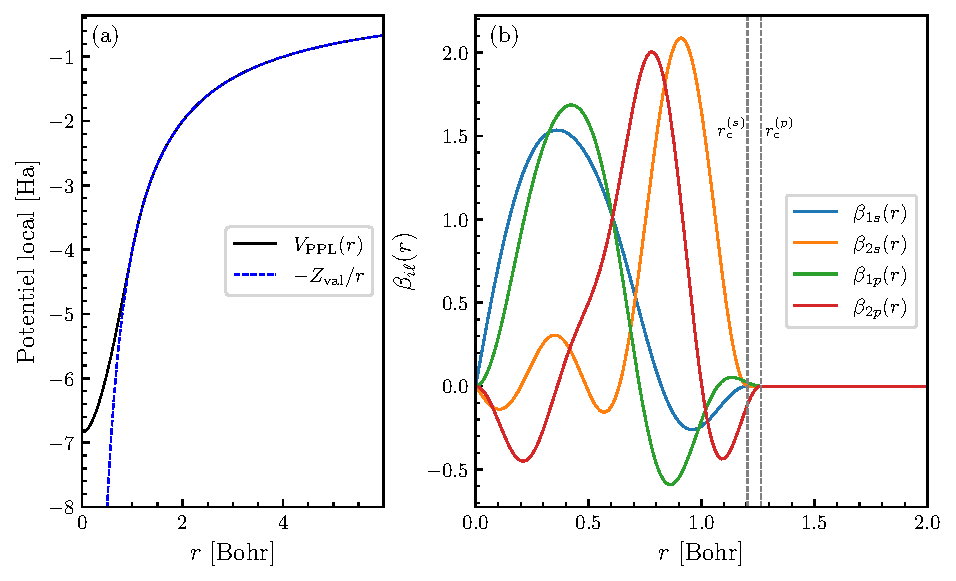
\includegraphics{figures/KB_projectors_C.pdf}
    \caption[llustration de la partie locale et non-locale du pseudo-potentiel pour un atome
    de carbone.]{Illustration de la partie locale et non-locale du pseudo-potentiel pour un atome de carbone. (a) Comparaison entre la partie locale du pseudo-potentiel $V_\text{PPL}(r)$ et le potentiel de Coulomb $-Z_\text{val}/r$ où $Z_\text{val}=4$ est la charge des électrons de valence du carbone. Notons que $V_\text{PPL}(r)$ corrige la divergence du potentiel de Coulomb à l'origine. (b) Partie radiale des projecteurs de KB $\beta_{i\ell}(r)$, qui s'annulent au-delà des rayons de coupure $r_c^{(s)}$ et $r_c^{(p)}$. Le
    pseudo-potentiel est de type ONCV \textit{stringent} pour la fonctionnelle XC PBE, tiré de la bibliothèque PseudoDojo 
    \cite{vansettenPseudoDojoTrainingGrading2018}.}
    \label{fig:KB}
\end{figure}

\subsection{Base d'ondes planes et résolution des équations de Kohn-Sham dans l'espace réciproque}\label{sec:PW}

Dans cette section, nous voyons comment résoudre les équations de Kohn-Sham en pratique dans l'espace réciproque. À cet effet, il est nécessaire de faire l'expansion de la fonction d'onde dans une base complète. Pour les solides cristallins, une base naturelle est celle des ondes planes, puisqu'elle exploite la symétrie de translation discrète des cristaux.

\noindent\textbf{Base d'ondes planes}

D'après le théorème de Bloch (cf. section~\ref{sec:2.1.2}), les fonctions d'onde de KS prennent la forme
\begin{equation}
    \psi_{n\kv}(\rv)=e^{i\kv\cdot\rv}u_{n\kv}(\rv),
    \label{eqn:c2_bloch_pt2}
\end{equation}
où la fonction périodique de Bloch possède la même périodicité que le solide : $u_{n\kv}(\rv+\Rv_\ell) = u_{n\kv}(\rv)$. Grâce à cette invariance sous translation discrète par un vecteur du réseau cristallin, il est possible de faire son expansion en série de Fourier avec les vecteurs $\Gv$ du réseau réciproque seulement
\begin{equation}
    u_{n\kv}(\rv)=\frac{1}{\sqrt{\Omega_\text{BvK}}}\sum_{\Gv}C_{n\kv}(\Gv)e^{i\Gv\cdot\rv},
    \label{eqn:c2_uPW}
\end{equation}
où $\Omega_\text{BvK}$ est le volume du cristal et $C_{n\kv}(\Gv)$ sont les coefficients de l'expansion en série de Fourier, de sorte que la fonction d'onde de KS s'écrit comme une combinaison linéaire d'ondes planes
\begin{equation}
    \psi_{n\kv}(\rv)=\frac{1}{\sqrt{\Omega_\text{BvK}}}\sum_{\Gv}C_{n\kv}(\Gv)e^{i(\kv+\Gv)\cdot\rv}.
    \label{eqn:c2_psiPW}
\end{equation}
La base d'onde plane est un choix naturel pour les solides périodiques : elle est complète, orthonormée, et compatible avec les transformées de Fourier rapides (FFT, de l'anglais \textit{Fast Fourier Transform}) qui permettent de passer efficacement entre l'espace réel et l'espace réciproque. Le problème se réduit donc à la détermination des coefficients $C_{n\kv}(\Gv)$.

Formellement, il faut un nombre infini d'ondes planes pour représenter la fonction d'onde. En pratique, nous tronquons la série en introduisant une énergie de coupure $E_\text{cut}$ telle que seules les ondes planes satisfaisant
\begin{equation}
    \frac{\hbar^2}{2m_e}|\kv+\Gv|^2\leq E_\text{cut}.
    \label{eqn:c2_Ecut}
\end{equation}
sont retenues. Une valeur de $E_\text{cut}$ plus élevée améliore la précision des calculs au prix d'un coût numérique plus grand. Notons qu'un très grand nombre d'ondes planes seraient nécessaires pour représenter les oscillations rapides des fonctions d'onde près des noyaux. Heureusement, ce problème est résolu par l'approximation des pseudo-potentiels (cf. section~\ref{sec:PP}), qui garantit des fonctions d'onde lisses dans la région de c\oe ur.

Finalement, nous souhaitons que les fonctions d'onde soient orthonormales sur l'ensemble du système, soit le volume du cristal $\Omega_\text{BvK}$ 
\begin{equation}
    \int_{\Omega_\text{BvK}}d^3\rv\,\psi_{n\kv}^*(\rv)\psi_{n'\kv'}(\rv)=\delta_{nn'}\delta_{\kv\kv'}.
    \label{eqn:c2_psi_norm}
\end{equation}
En remplaçant les fonctions d'onde par leur expansion en ondes planes \eqref{eqn:c2_psiPW}, nous pouvons montrer que les coefficients d'expansion satisfont la relation
\begin{equation}
    \sum_\Gv C_{n\kv}^*(\Gv)C_{n'\kv}(\Gv)=\delta_{nn'}.
    \label{eqn:c2_C_norm}
\end{equation}
Nous avons maintenant tous les ingrédients nécessaires pour écrire les équations de KS dans la base d'ondes planes et les résoudre formellement.

\noindent\textbf{Équations de Kohn-Sham dans la base d'ondes planes}

Nous souhaitons écrire les équations de KS (équations \eqref{eqn:c2_KS}--\eqref{eqn:c2_VKS}) dans la base d'ondes planes. Premièrement, en substituant la forme de Bloch pour la fonction d'onde, nous obtenons les équations de KS en termes de $u_{n\kv}(\rv)$,
\begin{equation}
    \left(-\frac{\hbar^2}{2m_e}(\nabla+i\kv)^2+V_\text{KS}(\rv)\right)u_{n\kv}(\rv)=\varepsilon_{n\kv}u_{n\kv}(\rv),
    \label{eqn:c2_UKS}
\end{equation}
Ensuite, en utilisant l'expansion de $u_{n\kv}(\rv)$ en ondes planes (équation \eqref{eqn:c2_uPW}) dans l'équation précédente et en utilisant l'expansion de $V_\text{KS}(\rv)$ en série de Fourier 
\begin{equation}
    V_\text{KS}(\rv)=\sum_{\Gv}\tilde{V}_\text{KS}(\Gv)e^{i\Gv\cdot\rv},
    \label{eqn:c2_VKSG}
\end{equation}
nous obtenons les équations de KS dans la base d'ondes planes
\begin{equation}
    \sum_{\Gv'}\left(\frac{\hbar^2}{2m_e}|\kv+\Gv|^2\delta_{\Gv\Gv'}+\tilde{V}_\text{KS}(\Gv-\Gv')\right)C_{n\kv}(\Gv')=\varepsilon_{n\kv}C_{n\kv}(\Gv).
    \label{eqn:c2_KSPW}
\end{equation}
Notons que l'expansion en série de Fourier du potentiel de KS ne se fait qu'avec les vecteurs du réseau réciproque $\Gv$, car $V_\text{KS}$ est aussi invariant sous une translation par un vecteur du réseau cristallin $\Rv_\ell$. L'équation de KS dans la base d'ondes planes, l'équation \eqref{eqn:c2_KSPW}, est formellement un problème aux valeurs propres matriciel $H^{(\kv)}_{\Gv\Gv'}\mathbf{C}=\varepsilon\mathbf{C}$, où la matrice Hamiltonienne est donnée par
\begin{equation}
    H^{(\kv)}_{\Gv\Gv'}=\frac{\hbar^2}{2m_e}|\kv+\Gv|^2\delta_{\Gv\Gv'}+\tilde{V}_\text{KS}(\Gv-\Gv').
    \label{eqn:c2_HGG}
\end{equation}
Cette matrice Hamiltonienne est de taille $N_\text{PW}\times N_\text{PW}$, où $N_\text{PW}$ est le nombre d'ondes planes déterminé par la coupure d'énergie cinétique $E_\text{cut}$ de l'équation \eqref{eqn:c2_Ecut} et dépend généralement du point $\kv$ considéré. Le paramètre $E_\text{cut}$ contrôle donc la taille du problème aux valeurs propres à résoudre à chaque itération du cycle SCF. En pratique, $N_\text{PW}$ peut atteindre plusieurs milliers à plusieurs dizaines de milliers d'ondes planes selon le système et la précision souhaitée. Notons également que la matrice Hamiltonienne dépend de $\kv$ et doit être construite pour chaque $\kv$ de la première IBZ. Le potentiel $\tilde{V}_\text{KS}(\Gv-\Gv')$ est mis à jour à chaque itération du cycle SCF à partir de la nouvelle densité $n_\text{out}(\rv)$ que nous décrivons en détail dans ce qui suit et est illustré à la figure \ref{fig:scf_PW}. Le cycle SCF dans la base d'ondes planes se déroule comme suit:
\begin{enumerate}
    \item Commencer avec une estimation de la densité initiale $n_\text{in}(\rv)$.
    \item Transformer la densité d'entrée dans l'espace réciproque à l'aide d'une FFT:
    \begin{equation*}
        n_\text{in}(\rv) \xrightarrow{\text{FFT}} \tilde{n}_\text{in}(\Gv).
    \end{equation*}
    \item Calculer les composantes de Fourier de la partie locale du potentiel de KS. La partie de Hartree est obtenue directement dans l'espace réciproque via l'équation de Poisson
    \begin{equation*}
        \tilde{V}_\text{H}(\Gv)=\frac{4\pi e^2}{|\Gv|^2}\tilde{n}_\text{in}(\Gv),
    \end{equation*}
    la partie d'échange-corrélation $\tilde{V}_\text{XC}(\Gv)$ est obtenue par la FFT de $V_\text{XC}[n_\text{in}(\rv)]$ calculé dans l'espace réel, et la partie locale du pseudo-potentiel $\tilde{V}_\text{PPL}(\Gv)$ est précalculée en faisant la FFT de $V_\text{PPL}(\rv)$, qui ne dépend pas de la densité. La partie locale est assemblée dans l'espace réciproque par la somme de ces trois termes
    \begin{equation*}
        \tilde{V}_\text{L}(\Gv) = \tilde{V}_\text{H}(\Gv)+\tilde{V}_\text{XC}(\Gv)+\tilde{V}_\text{PPL}(\Gv).
    \end{equation*}
    \item Précalculer la partie non-locale du potentiel de KS pour chaque $\kv$, car elle ne dépend pas de la densité
    \begin{equation*}
        \tilde{V}_\text{NL}^{(\kv)}(\Gv, \Gv')=\sum_\alpha\sum_{i\ell m}\tilde{\beta}_{i\ell m}^{(\alpha)}(\kv+\Gv)E_{i\ell}^{(\alpha)}\tilde{\beta}^{*(\alpha)}_{i\ell m}(\kv+\Gv').
    \end{equation*}
    La dérivation de cette expression est présentée dans le chapitre \ref{chap:défauts} dans le contexte du calcul des éléments de matrice électron-défaut.
    \item Construire la matrice Hamiltonienne pour chaque point $\kv$ de la première BZ
    \begin{equation*}
        H^{(\kv)}_{\Gv\Gv'}=\frac{\hbar^2}{2m_e}|\kv+\Gv|^2\delta_{\Gv\Gv'}+\tilde{V}_\text{L}(\Gv-\Gv')+\tilde{V}^{(\kv)}_\text{NL}(\Gv,\Gv'),
    \end{equation*}
    et diagonaliser pour obtenir les coefficients $C_{n\kv}(\Gv)$ et les valeurs propres $\varepsilon_{n\kv}$. La diagonalisation se fait itérativement à l'aide d'algorithmes de sous-espace tels que Davidson ou LOBPCG.
    \item Calculer les fonctions d'ondes dans l'espace réel à partir des coefficients des ondes planes à l'aide d'une FFT inverse
    \begin{equation*}
        C_{n\kv}(\Gv)\xrightarrow{\text{FFT}^{-1}}\psi_{n\kv}(\rv).
    \end{equation*}
    \item Calculer la nouvelle densité électronique à partir des fonctions d'onde dans l'espace réel
    \begin{equation*}
        n_\text{out}(\rv)=\sum_{n\kv}f_{n\kv}|\psi_{n\kv}(\rv)|^2,
    \end{equation*}
    où $f_{n\kv}$ est un facteur d'occupation.
    \item Construire la nouvelle densité d'entrée à partir de $n_\text{in}$ et $n_\text{out}$ via un schéma de \textit{mixing}, \textit{e.g.} Pulay ou DIIS.
    \item Si la différence entre $n_\text{in}$ et $n_\text{out}$ est inférieure à une tolérance spécifiée, ou d'autres critères de convergence sont satisfaits, passer à l'étape 10. Autrement, retourner à l'étape 2. 
    \item Calculer les propriétés de l'état fondamental.
\end{enumerate}
\noindent
\textbf{Schéma de \textit{mixing}}
\\
\noindent
\textbf{Facteur d'occupation et \textit{smearing}}
\\
\noindent
\textbf{Échantillonage de la zone de Brillouin}

\subsection{Résultats pour le graphène}
\section{Partie ionique : les phonons et la théorie de la fonctionnelle de la densité perturbative}
\label{sec:2.3}
À l'instar de son homologue électronique, le problème ionique n'est pas moins complexe à résoudre que le problème initial. Le coupable est encore une fois l'interaction mutuelle entre tous les ions qui se trouve dans le potentiel effectif $U$.
\subsection{Approximation harmonique}
\subsection{Quantification des vibrations du réseau : phonons}
\subsection{Théorie de la fonctionnelle de la densité perturbative}
\subsection{Résultats pour le graphène}

\section{Fonctions de Wannier}
\subsection{Définitions de base}
\subsection{Calculs des fonctions de Wannier}
\subsection{Interpolation de Wannier}

\section{Photons}
\subsection{Quantification du champ électromagnétique}
\subsection{Couplage électron-photon}
%\chapter{Fondements théoriques de la spectroscopie Raman}

\section{Théorie macroscopique semi-classique de la spectroscopie Raman}

\section{Théorie microscoscopique quantique de la spectroscopie Raman}
%\chapter{Couplage électron-défaut dans le graphène}
\label{chap:défauts}
%\chapter{Couplage électron-phonon dans le graphène}
\label{chap:eph}
%\chapter{Conclusion}

%%--------------%
%%     index    %
%%--------------%

%%\printindex

%%------------------------------------------------- %
%%                   Annexe                         %
%%------------------------------------------------- %

\appendix

\chapter{Dérivation des \textit{self}-énergies pour le couplage électron-phonon à partir de la théorie de la perturbation à plusieurs corps}
%\chapter{Dérivation de la matrice $T$ à partir de la théorie de la perturbation à plusieurs corps}
%\chapter{Paramètres utilisés dans les calculs numériques}
%\chapter{Paramètres utilisés dans les calculs numériques}

%\printbibliography
\end{document}
\endinput
